\documentclass{article}
\usepackage{ctex}
\usepackage{graphicx}

\usepackage{enumerate}
\usepackage[top=1cm]{geometry}
\graphicspath{{picture/}}
\title{HDFS分布式系统}
\author{W.J.Z}
\date{}
\begin{document}
	\maketitle
	分布式文件系统是一种通过网络实现文件在多台主机进行分布式储存的文件系统,分布式文件系统的设计一般采用“客户机/服务器”模式,客户端通过特定的通信协议与服务器建立连接,提出文件访问请求。
	\section{hdfs的特点}
	\begin{enumerate}
		\item 兼容廉价的硬件设备:hdfs可运行在廉价服务器上,并设计了快速检测硬件故障和进行自动恢复机制,使得在硬件出错情况下也能实现数据的完整性。
		\item 流数据读写:普通文件系统主要用于随机读写及与用户交互,而分布式系统HDFS是为了满足批量数据处理的要求而设计的。
		\item 大数据集:HDFS中的文件通常可以达到GB或TB级别。
		\item  简单文件模型:HDFS采用一次写入、多次读取的模型,写入时只支持单个写入者且写操作是以“只添加”方式在文件末尾写数据。
		\item 跨品台兼容性;HDFS采用java语言实现,支持JVM的机器都可以运行HDFS。	
		\item 不适合低延迟数据访问:HDFS主要针对大规模数据批量处理而设计的,延迟较高.		
		\item 不适用于存储小文件:小文件过多会造成存储在namenode节点内存中的元数据过多,造成元数据检索效率降低,同时内存空间需求量会大大增加;使用MapReduce处理大量小文件时,会产生过多的Map任务,线程管理开销会增加。
	\end{enumerate}
	\section{HDFS相关概念}
	\subsection{块}
	HDFS块的大小为128MB(以后随着硬盘容量的变大还会变),比磁盘块大,其目的是为了最小化寻址开销。如果块足够大,数据传输时间会明显的大于定位该块起始位置所需的时间。
	
	HDFS上的文件也被划分为块大小的多个分块,这样的好处:(1)、一个文件的大小可以大于网络中任意一个磁盘的大小;(2)、使用抽象块而非整个文件作为储存单元,大大简化存储子系统的设计。(3)、块适用于数据备份而提供数据容错能力和提高可用性。
	\subsection{namenode 和datanode}
	namenode负责管理分布式文件系统的命名空间,保存了两个核心的数据结构FsImage和EditLog,FsImage用于维护文件系统树以及文件树中所有的文件和文件夹的元数据,EditLog记录所有针对文件的创建、删除、命名等操作,这些信息以两个文本的形式永久的保存在本地磁盘上。namenode还记录每个文件中的各个块所在的数据节点信息,这些信息不会持久化保存,而在系统每次启动时扫描所有数据节点重构得到这些信息。 
	\subsection{secondarynamenode}
	一旦namenode失效,文件系统将无法工作,因此对namenode实现容错非常重要。secondarynamenode负责定期合并并编辑日志与命名空间镜像,以防止编辑日志过大。
	\begin{figure}[h]
		\centering
		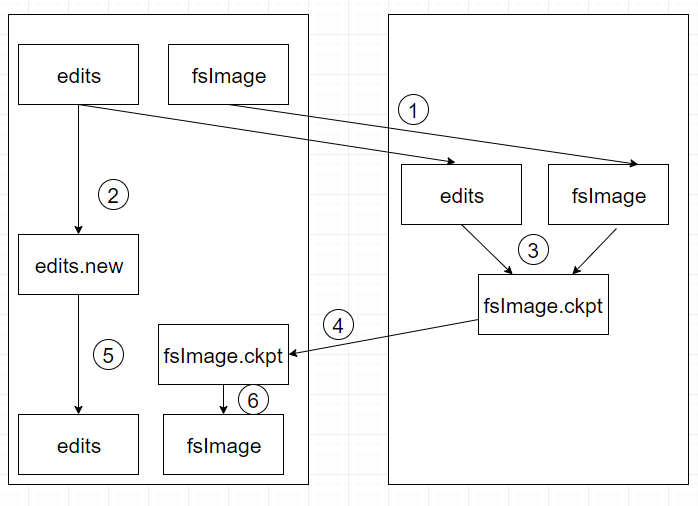
\includegraphics[scale=0.4]{1}
	\end{figure}
	\begin{enumerate}
		\item 使用http get复制edits和fsimage文件。
		\item 生成新的edits
		\item 将fsimage导入内存,应用edits中的操作,生成新的fsimage.ckpt。
		\item 使用http post发送fsimage.ckpt。
		\item 将edits替换为新的edits.new。
		\item 将fsimage替换为fsimage.ckpt。
	\end{enumerate}
	secondarynamenode请求namenode停止使用edits,暂时将新写操作放入一个新的文件中(edits.new).通过http get获取edits和fsimage,将它们加载到内存中完成一系列合并操作生成新的fsiamge,然后通过http post方式将新的fsimage发送给namenode。namenode获取到新的fsimage并代替原有的fsimage,并把edits.new变为edits。namenode和secondarynamenode一般放在不同的机器上,fs.checkpoint.period:默认是一个小时。fs.checkpoint.size:默认64MB。
	 
	\subsection{联邦HDFS}
	为了实现系统横向扩展,联邦HDFS允许系统通过添加nadenode实现扩展,每个namenode管理文件系统命名空间的一部分,比如一个namenode复杂管理/usr目录下的所有文件,一个namenode负责管理/share目录下的文件。
	\section{常用命令}
	\begin{enumerate}
		\item hadoop fs -ls:显示指定目录信息
		\item hadoop fs -cat : 将内容输出到标准输出
		\item hadoop fs -chgrp:改变文件所属的组
		\item hadoop fs -chown:改变文件的所有者
		\item hadoop fs -tail:将文件末尾内容输出到标准输出
		\item hadoop fs -mkdir:创建一个文件夹
		\item hadoop fs -copyFromLocal<local><dis>:将本地文件上传到分布式系统中
		\item hadoop fs -copyToLocal:将目标文件复制到本地系统中
		\item hadoop fs -cp<src><dis>:复制文件
		\item hadoop fs -get<src><local>:复制分布式系统中文件到本地系统
		\item hadoop fs -put<local><dis>:将本地系统文件复制到分布式系统中
		\item hadoop fs -mv:移动文件
		\item hadoop fs -rm:删除文件
		\item hadoop fs -test:检查文件相关信息,-e 文件是否存在,存在返回0,否则1;-z 文件是否为0字节,是返回0否则返回1;-d 路径是否是一个目录,是返回0否则返回1;
	\end{enumerate}
	\section{HDFS常用JAVA API及应用实例}
	\begin{enumerate}
		\item org.apache.hadoop.fs.FileSystem:一个通用文件系统的抽象基类,可以被分布式系统继承。
		\item org.apache.hadoop.fs.FileStatus:一个接口,向客户端展示系统中文件和目录的元数据。
		\item org.apache.hadoop.fs.FSDataInputStream:文件输入流,用于读取hadoop文件。
		\item org.apache.hadoop.fs.FSDataOutputStream:文件输出流,用于写hadoop文件。
		\item org.apache.hadoop.conf.Configuration:访问配置项。
		\item org.apache.hadoop.fs.Path:用于表示hadoop文件系统中的一个文件或一个目录。
		\item org.apache.hadoop.fs.PathFilter:一个接口,实现方法PathFilter.accpt(Path path)来决定是否接受路径path表示的文件或目录。
	\end{enumerate}
	 
\end{document}